\documentclass[10pt]{amsart}
\usepackage{amsmath}
\usepackage{amsfonts}
\usepackage{amssymb}
\usepackage{csquotes}
\usepackage{enumitem}
\usepackage{tikz}

\newtheorem{definition}{Definition}[section]

\newcommand{\w}{\wedge}
\newcommand{\p}{\partial}
\newcommand{\px}[1]{\partial_{x^{#1}}}
\newcommand{\py}[1]{\partial_{y^{#1}}}
\newcommand{\ra}{\rightarrow}
\newcommand{\dvol}{\text{dvol}_g}
\renewcommand{\hom}{\text{Hom}}
\newcommand{\im}{\text{Im}}
\renewcommand{\ker}{\text{Ker}}
\newcommand{\id}{\text{Id}}
\newcommand{\C}{\mathcal{C}}
\newcommand{\ob}{\mathcal{O}}
\newcommand{\obj}{\text{Obj}}
\newcommand{\M}{\mathcal{M}}
\newcommand{\R}{\mathbb{R}}
\newcommand{\vp}{\varphi}
\renewcommand{\o}{\circ}
\renewcommand{\i}{^{-1}}
\renewcommand{\a}{\alpha}
\renewcommand{\b}{\beta}
\newcommand{\rmg}{\sqrt{\left\vert g\right\vert}}
\newcommand{\wfb}{dx^1\wedge\cdots\wedge dx^n}
\newcommand{\wfby}{dy^1\wedge\cdots\wedge dy^n}
\newcommand{\tvs}{V_1\ox\cdots\ox V_n}
\newcommand{\wvs}{V\wedge\cdots\wedge V}
\newcommand{\x}{\times}
\renewcommand{\*}{\star}
\newcommand{\ox}{\otimes}
\newcommand{\pder}[2]{\frac{\partial #1}{\partial #2}}

\title{Real Analysis II}
\author{Arden Rasmussen}
\date{\today}

\begin{document}
\maketitle

\section{Category Theory}%
\label{sec:category_theory}

\subsection{Category}%
\label{sub:category}

Category is a pair of objects and morphisms
\begin{align*}
  \C=(\ob,\M)
\end{align*}

\subsubsection{Examples}%
\label{ssub:examples}

\begin{itemize}
  \item (Vector Spaces, Linear Transformations)
  \item (Metric Spaces, Continuous Maps)
  \item (Manifolds, Differentiable Maps)
\end{itemize}

\subsubsection{Homeomorphisms}%
\label{ssub:homeomorphisms}

\begin{align*}
  \hom(\ob_1,\ob_2)
\end{align*}
This is all okay functions between $\ob_1$, and $\ob_2$.

\begin{align*}
  \id&(\ob)=\ob\\
  f\o\id=&f=\id\o f\\
  \left(f\o g\right)\o h&=f\o\left(g\o h\right)
\end{align*}

\begin{definition}
  $f\in\hom\left(\obj_1,\obj_2\right)$ is an \textit{isomorphism} if $\exists
    f\i\in\hom\left(\obj_2,\obj_1\right)$ with $f\o f\i=\id=f\i\o f$.
\end{definition}

\subsection{Functors}%
\label{sub:functors}

\begin{definition}
  $F:\C_1\ra\C_2\quad\forall\ \obj\in\C_1\ \exists\ \obj\in\C_2$. With
  $F(\id)=\id$, and $F(T\o L)=F(T)\o F(L)$ (or $F(T\o L)=F(L)\o F(T)$).
  This means that identity and compositions are preserved. Functors can either
  be covariant or contravairant.
\end{definition}

Covariant functors push morphisms forwards, contravariant pull morphisms back.

\begin{figure}[htpb]
\begin{center}
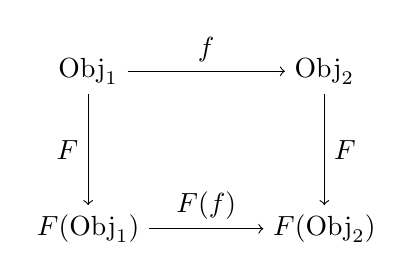
\begin{tikzpicture}[scale=1, transform shape]
  \node (a) at (0,2) {$\obj_1$};
  \node (b) at (3,2) {$\obj_2$};
  \node (c) at (0,0) {$F(\obj_1)$};
  \node (d) at (3,0) {$F(\obj_2)$};
  \draw [->](a) -- node[above]{$f$} (b);
  \draw [->](a) --node[left]{$F$} (c);
  \draw [->](b) --node[right]{$F$} (d);
  \draw [->](c) --node[above]{$F(f)$} (d);
\end{tikzpicture}
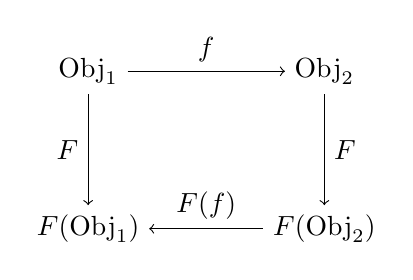
\begin{tikzpicture}[scale=1, transform shape]
  \node (a) at (0,2) {$\obj_1$};
  \node (b) at (3,2) {$\obj_2$};
  \node (c) at (0,0) {$F(\obj_1)$};
  \node (d) at (3,0) {$F(\obj_2)$};
  \draw [->](a) -- node[above]{$f$} (b);
  \draw [->](a) --node[left]{$F$} (c);
  \draw [->](b) --node[right]{$F$} (d);
  \draw [<-](c) --node[above]{$F(f)$} (d);
\end{tikzpicture}
\end{center}
\caption{covariant and contravariant functors}
\label{fig:functors}
\end{figure}

\subsubsection{Examples}%
\label{ssub:examples}

Exterior powers:
$V\mapsto\Lambda^k(V)$ is a functor.

\subsection{Cohomology Functor}%
\label{sub:cohomology_functor}

If $F:\M_1\ra\M_2$ then $F^*:\Gamma(\Lambda^k(M_2))\ra\Gamma(\Lambda^k(\M_1))$.
We use this functor to determine if manifolds are the same. However it is only
one directional. If $\M_1\cong\M_2\implies H^k(\M_1)\cong H^k(\M_2)$.

So since $H^0([0,1])\ncong H^0(S^1)$, then we know that $[0,1]\ncong S^1$. The
same applies for $T^2$ and $S^2$ just using $H^1$.

To show that there is no smooth functions, assume there is, and then show that
the dimensions don't match up of $H^1$, and so there is nonsense, so that
becomes a contradiction.

\subsection{Algebraic Topology}%
\label{sub:algebraic_topology}

Functor from category of manifolds to vector spaces, ``measuring'' the manifold
by associating vector spaces to it. Then work can be done on the vector spaces,
which is much simpler than to do it on the manifolds.

\section{Manifolds}%
\label{sec:manifolds}

\subsection{Definition of Manifold}%
\label{sub:definition_of_manifold}

\begin{definition}
  A metric space $(\M,d)$ is said to be a $n$-dimensional manifold if there
  exists a collection of mappings $\left\{\vp:U_\vp\ra\M\right\}$. Such that if
  $\vp(U_\vp)=V\vp$ then
  \begin{itemize}
    \item $U_\vp\subseteq \R^n$
    \item $\vp:U_\vp\ra\vp(U_\vp)\subseteq\M$ is a homeomorphism. (Continuous
      mapping with continuous inverse).
    \item $\bigcup_\vp V_\vp=\M$
    \item For all $\vp_1,\vp_2\in\left\{\vp\right\}$ we have
      \begin{align*}
        \vp_2\i\o\vp_1:\vp_1\i(V_{\vp_1}\cap V_{\vp_2})\ra\vp_2\i(V_{\vp_1}\cap V_{\vp_2})
      \end{align*}
      is a diffeomorphism. $\vp_2\i\o\vp_1$ are called transition maps.
  \end{itemize}
\end{definition}

These are all manifolds, because they can be paramatrixes with some number of
bijective maps. For $S^1$ we use the angle, but need to to cover the point of
where $\theta$ is discontinuous. So we get
\begin{align*}
  \vp_1&:(-\pi,\pi)\ra S^1&\quad&\vp_0(t)=(\cos(t),\sin(t))\\
  \vp_2&:(0,2\pi)\ra S^1&\quad&\vp_0(t)=(\cos(t),\sin(t))\\
\end{align*}

\subsection{Orientability}%
\label{sub:orientability}

\begin{definition}
  A manifold is called orientable if there is an atlas of charts
  $\left\{\vp:U_\vp\ra\M\right\}$ covering $\M$ such that each function
  $\Phi_x^y:=\vp_2\i\o\vp_1$ has a positive Jacobian
  $\det\left[D\Phi_x^y\right]$. In these notes we will use the phrase
  orientable atlas when we refer to an atlas in which transitions functions
  always have positive Jacobian.
\end{definition}

\begin{definition}
   A manifold is called orientable if it permits a nowhere vanishing n-form.
\end{definition}

These two definitions are equivalent. Suppose $\omega$ is a nowhere vanishing
volume form on $\M$. Then for any parametrization $\vp(x^1,\ldots,x^n)$ we have
\begin{align*}
  \omega(\px{1},\ldots,\px{n})\wfb\neq 0.
\end{align*}
By swapping $x^1$ and $x^2$ variables in the parametrization (if necessary!) we
can in fact ensure that
\begin{align*}
  \omega(\px{1},\ldots,\px{n})>0
\end{align*}
for all $\vp$. Given two overlapping parametrizations we have the relationship
\begin{align*}
  \omega(\px{1},\ldots,\px{n})=\det\left[D\Phi_x^y\right]\omega(\py{1},\ldots,\py{n}),
\end{align*}
which then further implies
\begin{align*}
  \det\left[D\Phi_x^y\right]>0
\end{align*}
for all transition function $\Phi_x^y$. In other worlds, if a manifold is
orientable according to the second definitions it is also orientable according
to the first definition.

To prove the converse we use $\dvol$, we note that
$g_{kl}=\sum\pder{x^i}{y^k}\pder{x^j}{y^l}g_{ij}$. By taking the determinant,
we can then get rid of the absolute values, by our assumption. We then have
\begin{align*}
  \wfby=\det\left[D\Phi_x^y\right]\wfb.
\end{align*}
Then using chain rule we get $\dvol$ on both $y$ and $x$. Since this is
coordinate invariant, and will always be positive, then it is defined on $\M$,
and is non vanishing.

\subsubsection{Examples}%
\label{ssub:examples}

Most other manifolds, take the sphere for example. You can construct a nowhere
vanishing n-form to the sphere, it would be something like $\p r$, or something
of that sort.

\subsubsection{Non-Examples}%
\label{ssub:non_examples}

M\"obuis band. If you follow a normal vector all the way around the manifold,
at some point you will wrap back around to your self, but be pointing the other
way. This means that at some point the normal vector field must have passed
through zero, and so it vanishes. So this is not orientable.

\subsection{Tangent Vector and Tangent Space}%
\label{sub:tangent_vector_and_tangent_space}

$\gamma(t)$ on $\M$ is smooth mapping $\gamma:I\ra\M$. Let $f:\M\ra\R$ be some
observable. $f\o\gamma:I\ra\R$ is $f$ as observed by $\gamma$, so $\gamma$s
going in different directions should observe different rates of change of $f$
with $\pder{}{t}\Bigr|_{t=0}(f\o\gamma)$ being perceived rate of change.

We then say
\begin{align*}
  \gamma_1\sim\gamma_2\iff\pder{}{t}\Bigr|_{t=0}(f\o\gamma_1)=\pder{}{t}\Bigr|_{t=0}(f\o\gamma_2)
\end{align*}

The tangent space of $M$ at $P$ is the set of equivalence classes of curves at
$p$. All of the tangent vectors to $M$ at $P$.

\subsection{Cotangent Vector Field}%
\label{sub:cotangent_vector_field}

Cotangent vector field is a section of the cotangent bundle. A section is a
mapping such that each point of a subset of the manifold stays within the
associated vector space based at that point on the manifold. For the circle and
cylinder, a section $s$ can move point up and down, but not around the
cylinder. This way $\pi$ will bring the points back to the starting point. We
can write this as $\pi\o s=\id$.

\subsection{Tangent Bundle}%
\label{sub:tangent_bundle}

The tangent bundle is the disjoint union of the tangent space at all points on
the manifold. $\dim(TM)=2n$. Think of this like the cylinder to the
circle(Although this is not tangent).

There exists a projection map, that takes any point in a tangent space and
projects it to the base point $P$ that the tangent space is tangent to. This is
called $\pi$.

\subsection{$M\ra TM$}%
\label{sub:_mra_tm_}

Yes, $M\ra TM$ will result in getting something like $[\gamma]\ra[F\o\gamma]$.
Where $F$ is the ``functor''. This proves that this is a covariant functor?????

\section{Universal Property}%
\label{sec:universal_property}

\begin{definition}[Exterior Powers]
   Let $V$ be a vector space. By the $k$-th exterior power of $V$ we mean the
   vector space $E^k$ together with an alternating multilinear map
   $a:V\x V\x\ldots\x V\ra E^k$ (on $k$ copies of $V$) such that for each
   alternating multilinear map $\omega:V\x V\x\ldots\x V\ra W$ there exists a
   \textbf{unique} linear map $L:E^k\ra W$ for which $w=L\o a$.
\end{definition}

\begin{figure}[htpb]
\begin{center}
\begin{tikzpicture}[scale=1, transform shape]
  \node (a) at (0,3) {$V_1\x V_2\x\ldots\x V_n$};
  \node (b) at (0,0) {$V_1\ox V_2\ox\ldots\ox V_n$};
  \node (c) at (5,3) {$W$};
  \draw [->] (a) --node[above]{$\omega$} (c);
  \draw [->] (a) --node[left]{$b$} (b);
  \draw [dashed,->] (b) --node[below,right]{$\exists ! L$} (c);
\end{tikzpicture}
\end{center}
\caption{Universal property for tensor products of vector spaces
         $V_1,\ldots,V_n$.}
\label{fig:universal_prop}
\end{figure}

The universal property can be applied to different functors, so it can be used
for $\ox$, and for $\wedge$.


\section{Tensor Algebra}%
\label{sec:tensor_algebra}

\subsection{Using Universal Property}%
\label{sub:using_universal_property}

\begin{center}
\begin{tikzpicture}[scale=1, transform shape]
  \node (a) at (0,3) {$V^*\x V$};
  \node (b) at (0,0) {$V^*\ox V$};
  \node (c) at (5,3) {$\R$};
  \draw [->] (a) --node[above]{$\omega(\eta,v)=\eta(v)$} (c);
  \draw [->] (a) --node[left]{$b$} (b);
  \draw [dashed,->] (b) --node[below,right]{$\exists ! L$} (c);
\end{tikzpicture}
\end{center}

This proves that there must be some linear mapping $L$ that satisfies this.
This mapping is called the contraction operation.

\subsection{Basis and Dimension}%
\label{sub:basis_and_dimension}

The basis for $\tvs$ is going to be
\begin{align*}
  \left\{\px{i_1}\ox\cdots\ox\px{i_n}\right\}
\end{align*}
where the $\px{i_j}$ basis vector is a basis for the $V_j$ vector space.

The dimension of $\tvs$ is going to be the product of the dimensions of each
individual vector spaces.
\begin{align*}
  \dim(\tvs)=\dim(V_1)\dim(V_2)\cdots\dim(V_n)
\end{align*}

\subsection{Change of Basis}%
\label{sub:change_of_basis}

\begin{align*}
  T^{i_1\ldots i_p}_{j_1\ldots
  j_q}\px{i_1}\ox\ldots\ox\px{i_p}\ox dx^{j_1}\ox\ldots\ox dx^{j_q}
\end{align*}
\begin{align*}
  T^{\a_1\ldots \a_p}_{\b_1\ldots
  \b_q}=\sum
  T^{i_1\ldots i_p}_{j_1\ldots
  j_q}\pder{y^{\a_1}}{x^{i_1}}\cdots\pder{y^{\a_p}}{x^{i_p}}\pder{x^{j_1}}{y^{\b_1}}\cdots\pder{x^{j_q}}{y^{\b_q}}
\end{align*}

\subsection{Tensor Bundles and Sections}%
\label{sub:tensor_bundles_and_sections}

A Tensor bundle is gotten, by doing tensor products and such of each individual
$T_PM$ and by then taking the union over all $P$ gives us a tensor bundle of
sorts. Sections of it are tensor fields.

Tensor bundles are
\begin{align*}
  ((\ox^p)T^*M)\ox((\ox^q)TM)
\end{align*}

Tensor fields can be expressed as
\begin{align*}
  T=\sum T^{j_1\ldots j_q}_{i_1\ldots i_p}dx^{i_1}\ox\ldots\ox
  dx^{i_p}\ox\px{j_1}\ox\ldots\ox\px{j_q}
\end{align*}

\subsection{Mapping between Tensor Bundles}%
\label{sub:mapping_between_tensor_bundles}

\begin{center}
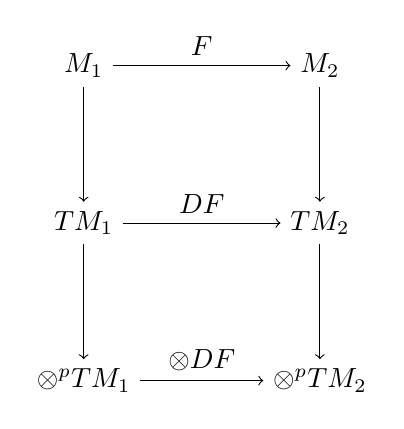
\begin{tikzpicture}[scale=1, transform shape]
  \node (a) at (0,2) {$M_1$};
  \node (b) at (3,2) {$M_2$};
  \node (c) at (0,0) {$TM_1$};
  \node (d) at (3,0) {$TM_2$};
  \node (e) at (0,-2) {$\ox^pTM_1$};
  \node (f) at (3,-2) {$\ox^pTM_2$};
  \draw [->](a) -- node[above]{$F$} (b);
  \draw [->](a) -- (c);
  \draw [->](b) -- (d);
  \draw [->](c) --node[above]{$DF$} (d);
  \draw [->](c) -- (e);
  \draw [->](d) -- (f);
  \draw [->](e)--node[above]{$\ox DF$} (f);
\end{tikzpicture}
\end{center}


\section{Exterior Calculus}%
\label{sec:exterior_calculus}

\subsection{Exterior Product on the Level of Linear Algebra}%
\label{sub:exterior_product_on_the_level_of_linear_algebra}

$\wedge$ can be though of as giving us the parallelotope spanned by the wedges
vectors. It is defined by determinant. The basis of $\wvs$ is
\begin{align*}
  dx^{i_1}\wedge\ldots\wedge dx^{i_k}\quad\text{for}\ 1\leq
    i_1<i_1<\cdots<i_k\leq n.
\end{align*}
This means that the dimension of the exterior product will be $n$ choose $k$.
Things change under diffeomorphism, by the determinant of the map. For change
of basis, this is the determinant of the transition map.

\subsection{Bundles and $k$-forms}%
\label{sub:bundles_and_k_forms}

\subsection{$\dvol$}%
\label{sub:_dvol_}

\begin{definition}
   \begin{align*}
     \dvol=\rmg\wfb
   \end{align*}
\end{definition}

$\dvol$ can be used to find the ``volume'' of a parallelotope. It only exists
if a manifold is orientable, and if we have a definition of $g$.

\subsection{Integration of $n$-forms on $n$-dimensional Manifolds}%
\label{sub:integration_of_n_forms_on_n_dimensional_manifolds}

\subsection{Flux Integration}%
\label{sub:flux_integration}

\subsubsection{Circulation Integrals}%
\label{ssub:circulation_integrals}

1-form to circulation integrals
\begin{align*}
  \int_\gamma\omega=\int_{t_i}^{t_f}\omega(\p_t)dt
\end{align*}
raising an index:
\begin{align*}
  \omega^\sharp=\vec{v}\implies\omega(\p_t)=g(\vec{v},\p_t)dt
\end{align*}
so we have:
\begin{align*}
  \int_\gamma\omega=\int_{t_i}^{t_f}g(\vec{v},\p_t)dt=\int_\gamma
  g(\vec{v},\vec{T})ds
\end{align*}
therefore, we set
\begin{align*}
  \int_\gamma \omega\leftrightarrow\int_\gamma\vec{v}\vec{T}ds
\end{align*}

\subsubsection{Flux Integrals}%
\label{ssub:flux_integrals}

1-form in 2d to flux
Suppose $\Sigma\subseteq M$( a curve on manifold ), $M$ is 2d. Assume
counter-clockwise Euclidean $\R^2$. Suppose $\omega$ is 1-form.

First, note that
\begin{align*}
  \omega(\p_t)dt=\omega(\vec{T})ds\\
  \vec{N}=(\*\vec{T})^\sharp
\end{align*}
Since $\*$ is isomorphism, we have
\begin{align*}
  -\omega=\*(\vec{v})
\end{align*}
for some vector field $\vec{v}$. Hence we set
\begin{align*}
  \omega(\vec{T})=-\dvol(\vec{v},\vec{T})=\dvol(\vec{T},\vec{v})=g(\vec{N},\vec{V})
\end{align*}
This is the flux integral we learned in calc III.

2-form in 3d. Suppose $\Sigma\subseteq M$, an oriented surface, $M$ is 3d,
$\omega$ is a 2-form. We know that
\begin{align*}
  \omega(\vec{V_1},\vec{V_2})=g(\vec{V_1},\vec{V_1}\times\vec{V_2})
\end{align*}
where $\vec{V}=\*\omega$
\begin{align*}
  \omega(\p_{u^1},\p_{u^2})&=\*(\vec{v})(\p_{u^1},\p_{u^2})\\
                           &=\dvol(\vec{v}, \p_{u^1},\p_{u^2})\\
                           &=\dvol(\p_{u^1},\p_{u^2},\vec{v})\\
                           &=g(\p_{u^1}\times\p_{u^2},\vec{v})\\
                           &=g(\vec{N},\vec{v})\sqrt{\det(\sim)}\\
                           &=g(\vec{N},\vec{V})dA
\end{align*}
Hence we set
\begin{align*}
  \int_\Sigma\omega=\int_\Sigma g(\vec{v},\vec{N})dA
\end{align*}
Flux of $\vec{V}$ across $\Sigma$

\subsection{Exterior Derivative}%
\label{sub:exterior_derivative}

\begin{align*}
  d\omega=\sum d\omega_{i_1\ldots i_k}\wedge dx^{i_1}\wedge\ldots\wedge dx^{i_k}
\end{align*}

$d$ is only thing that has the following properties
\begin{enumerate}
  \item $df$ is $d:\Gamma(\Lambda^0)\ra\Gamma(\Lambda^1)$ where $df$ is 1-form
    \begin{align*}
      df=\sum df(\px{i})dx^i=\sum\pder{(f\o\vp\i)}{x^i}dx^i
    \end{align*}
  \item $d$ distributes over $+$ and scalar.
  \item
    $d(\omega\wedge\eta)=d\omega\wedge\eta+(-1)^{\text{deg}(\omega)}\omega\wedge
    d\eta$
  \item $d^2\omega=0$
\end{enumerate}

\begin{align*}
  \vec{grad}f&=(df)^\sharp\\
  df(\vec{v})&=\sum\pder{f}{x^i}dx^i(\vec{v})=\sum\pder{f}{x^i}v^i\\
  d\omega(\vec{v})&=\*\o d\o\*(\vec{v})\\
  \text{curl}(\vec{v})&=\*\o d\o\flat(\vec{v})
\end{align*}

\subsection{Stokes' Theorem}%
\label{sub:stokes_theorem}

\subsection{Green-Gauss-Stokes' Theorems}%
\label{sub:green_gauss_stokes_theorems}

\begin{align*}
  \int_\Sigma \text{div}(\vec{v})dA&=\int_\Sigma d\omega\quad \text{where
  $d\omega=\*\vec{v}$}\\
                                   &=\int_\gamma\omega\\
                                   &=\int_\gamma\*\vec{v}(\p_t)dt\\
                                   &=\int_\gamma\*\vec{v}(\vec{T})ds\\
                                   &=\int_\gamma\dvol(\vec{v},\vec{T})\\
                                   &=-\int_\gamma\dvol(\vec{T}, \vec{v})\\
                                   &=-\int_\gamma\*\vec{T}(\vec{v})ds\\
                                   &=-\int_\gamma g(\*\vec{T}_\flat,
                                   \vec{v})ds\\
                                   &=\int_\gamma g(\vec{v},
                                   \vec{N}ds)\quad\text{Since
                                   $\*\vec{T}_\flat=-\vec{N}$}
\end{align*}

Greens
\begin{align*}
  \int_Md\omega=\int_{\p M}\omega\\
  \int_\M g(\* d\omega, \vec{N})dA=\int_{\p M}\omega(\p_t)dt\\
  \int_Mg(\* d\flat \vec{v},\vec{N})dA=\int_{\p M}g(\vec{v},\p_t)dt\\
  \int_Mg(\text{curl}\vec{v},\vec{N})dA=\int_{\p M}g(\vec{v},\vec{T})ds
\end{align*}

Stokes
\begin{align*}
  d\omega&=(-1)^{i-1}\p{f}{x^i}dx^1\wedge\ldots\wedge dx^n\\
  \int_M d\omega&=\int_{U_\vp}(-1)^{i-1}\p{f}{x^i}dx^1\ldots dx^n\\
                &=0\quad\text{unless $U_\vp$ hist the boundary}\\
                &=\int_{\p M}\omega
\end{align*}

\section{Cohomology}%
\label{sec:cohomology}

\subsection{Cochain Complex}%
\label{sub:cochain_complex}

\begin{align*}
  0\xrightarrow{d}\Gamma(\Lambda^0(T^*M))\xrightarrow{d}\Gamma(\Lambda^1(T^*m))\xrightarrow{d}\cdots
  \xrightarrow{d}\Gamma(\Lambda^n(T^*M))\xrightarrow{d}0.
\end{align*}

\begin{definition}
  Forms in $\ker(d)$ are called closed forms, and forms in $\im(d)$ are called
  exact forms.
\end{definition}

\begin{definition}
  The k-th cohomology of $\M$, denoted $H^k(\M)$, is the quotient vector space
  \begin{align*}
    H^k(\M)=\ker(d^k)/\im(d^{k-1}).
  \end{align*}
\end{definition}

In other words $H^k(\M)$ consists of equivalent classes of k-forms $\omega$ for
which
\begin{align*}
  d\omega
  =0\quad\text{under}\quad\omega_1\sim\omega_2\leftrightarrow\exists\eta,\quad
  \omega_1-\omega_2=d\eta.
\end{align*}

\subsection{Functorial Nature}%
\label{sub:functorial_nature}

Closed forms pull back to closed forms, and exact forms pull back from exact
forms, allows $H^k$ to be a functor. This is reliant on
\begin{align*}
  d(F^*\omega)=F^*d\omega.
\end{align*}
It is a contravariant functor.

\subsection{$H^0(\M)$}%
\label{sub:_h_0_m_}

This ``counts'' the number of path connected components in the manifold $\M$.
We did this proof as homework. Generally it goes as we know that $df=0$. So $f$
must be constant locally. Then because of path conceitedness it must be
constant on the entirety of the connected component. But for multiple
components, then each component can be its own constant.

Let $\M$ be a manifold, let $d$ be the number of its connected components.
Then $H^0(\M)\cong \R^d$.

\subsection{$d\theta$ on $S^1$}%
\label{sub:_dtheta_on_s_1_}

$d\theta$ is a special function, such that there does not exist any function
$f$ such that $df=d\theta$. This will result in $H^1(S^1)\cong\R$.

\subsection{$H^1(\M)$}%
\label{sub:_h_1_m_}

$H^1(\M)$ gives us the ``number of ways that $\M$ wraps in on itself''.

\subsection{Scalar and Vector Potentials}%
\label{sub:scalar_and_vector_potentials}

\end{document}
